\section{Introduction}
\label{sec:introduction}

As frontier AI systems are pretrained on web-scale data, test set contamination has become a critical concern for accurately assessing their capabilities \citep{sainz2023nlp,schaeffer2023pretrainingtestsetneed,xu2024benchmarkdatacontaminationlarge,deng2024unveiling,reuel2025open}.
Evaluation aims to measure generalization on tasks the model has never seen, yet the sheer scale of modern pretraining makes such contamination highly likely \citep{brown2020language, du2022glam, wei2022finetuned,chowdhery2022palmscalinglanguagemodeling,touvron2023llama2openfoundation, penedo2024finewebdatasetsdecantingweb}.

Prior research has sought to quantify the impact of test set contamination, also known as leakage, through two primary lenses. \textit{Statistical approaches} attempt to detect contamination or estimate its influence by modifying the test set, for example, by reordering, rephrasing, or replicating benchmark problems, e.g., \citep{oren2023proving, ni2025trainingbenchmarkneed, shi2024detecting, golchin2023data,golchin2024time,roberts2024to, wang2025generalization, zhang2024carefulexaminationlargelanguage}.
In comparison, \textit{controlled approaches} -- which enable the most direct causal measurement -- intentionally contaminate pretraining corpora to quantify how specific doses of leakage inflate performance, e.g., \citep{magar2022data,jiang2024investigatingdatacontaminationpretraining,oren2023proving,yao2024data, duan2024membership,wang2025generalization,kocyigit2025overestimation,bordt2025howmuch, wei2025hubblemodelsuiteadvance}.
For more, see Appendix~\ref{app:sec:related_work} Related Work.

\begin{figure*}[t!]
\centering
\hspace{-1em}
\begin{minipage}[t]{0.47\textwidth}
    \vspace{0pt}
    \centering
    % 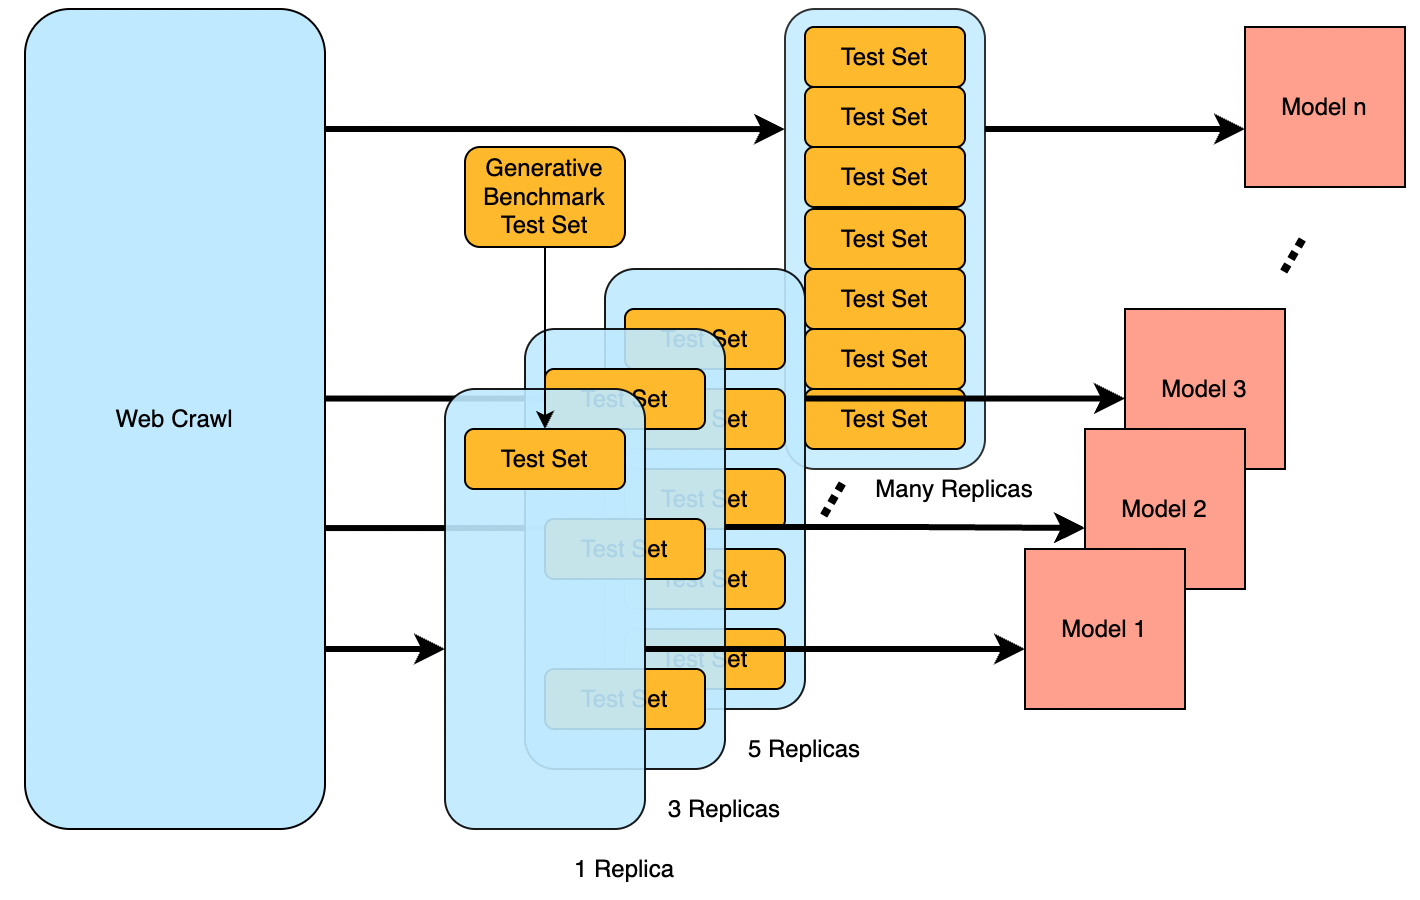
\includegraphics[width=\linewidth]{figures/01_revised_figures/pretraining_schematic.png}
    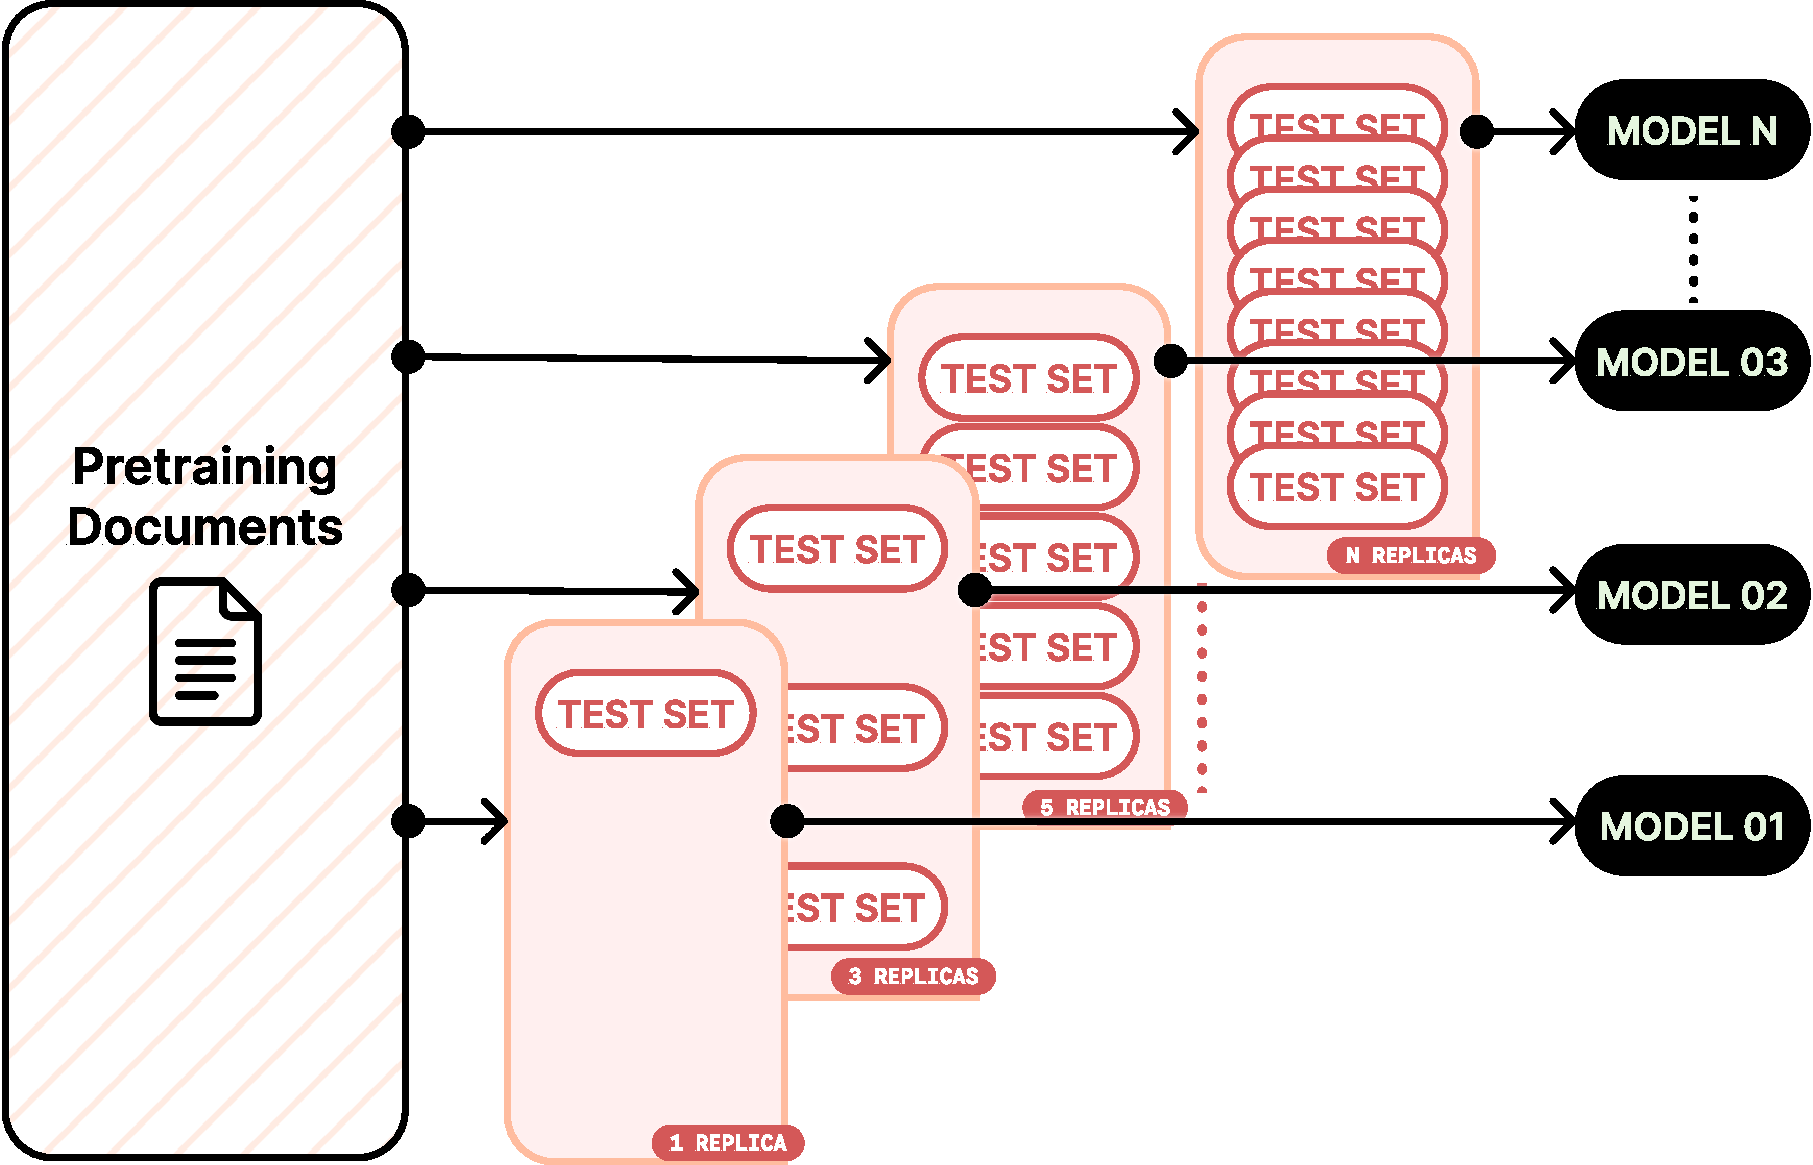
\includegraphics[width=\linewidth]{figures/schematic.pdf}
\end{minipage}%
\hspace{0.1em}
\begin{minipage}[t]{0.49\textwidth}
    \vspace{0pt}
    \centering
    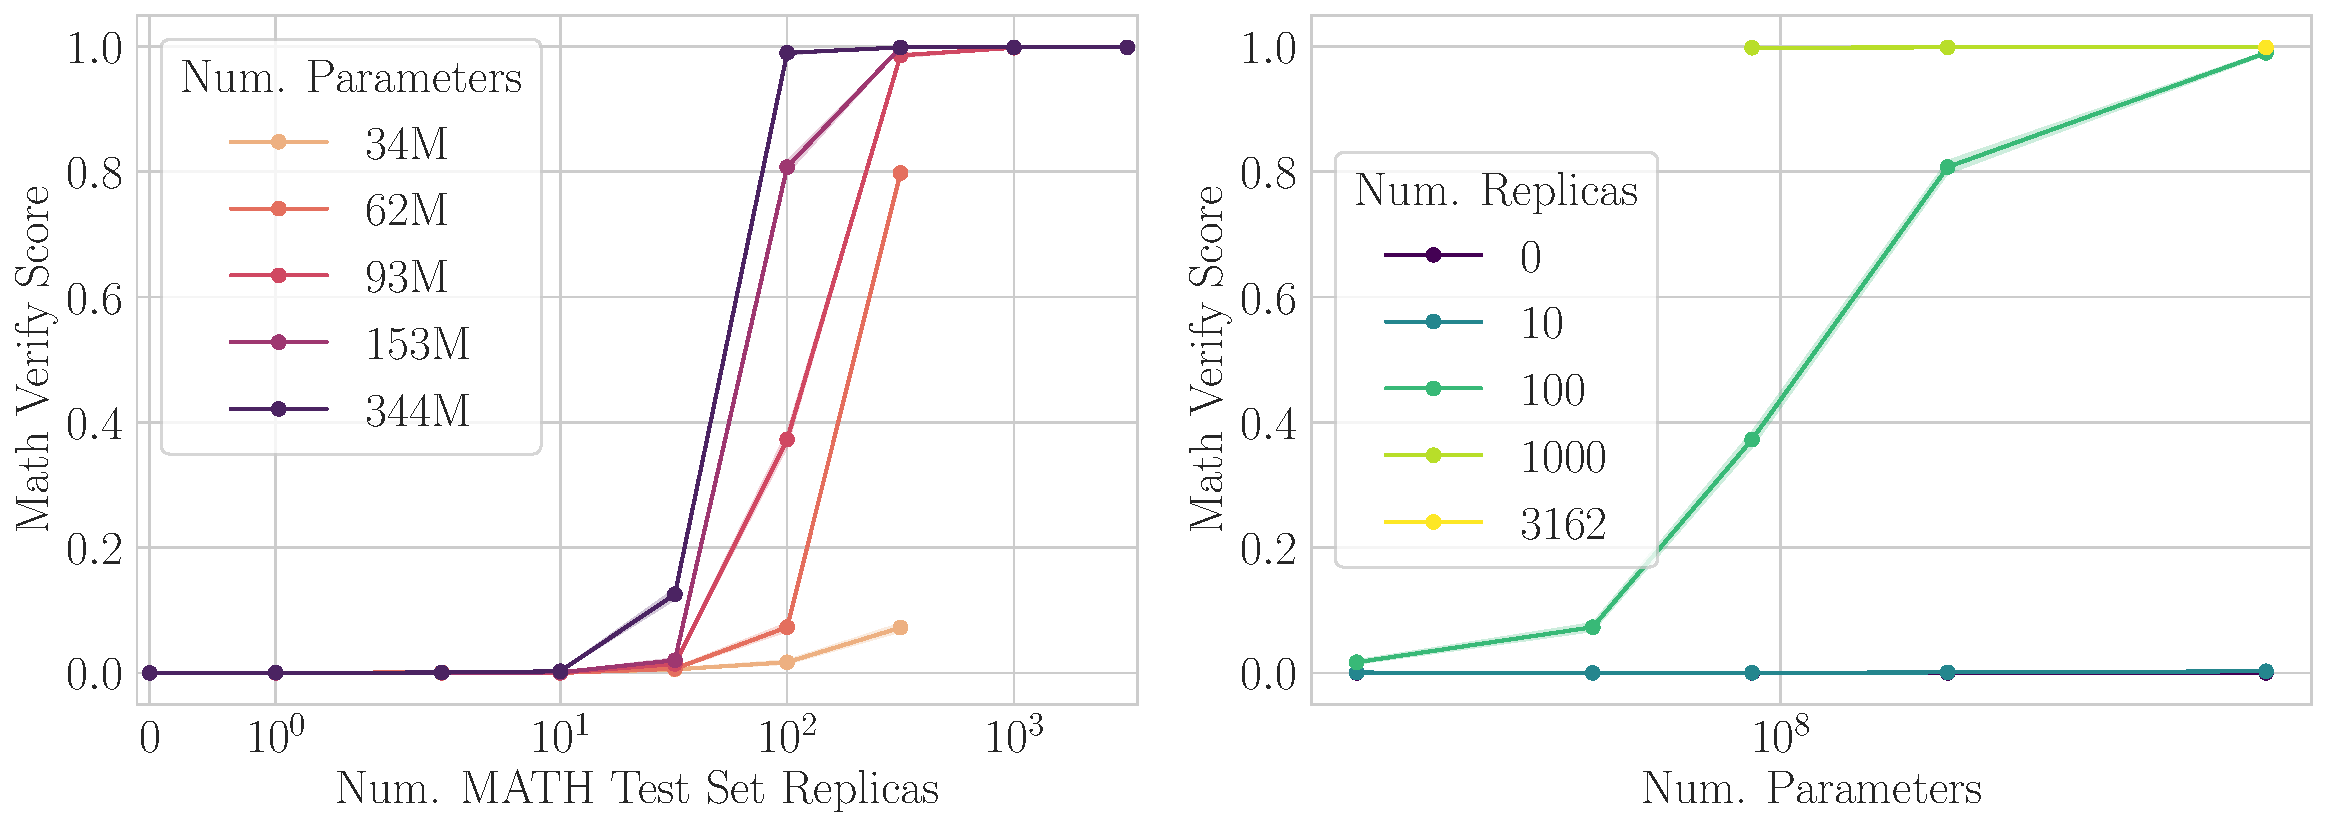
\includegraphics[width=\linewidth]{figures/11_math_qwen3_pt_math_verify/y=math_verify_strict_by_num_parameters_by_num_replicas.pdf}    
    % 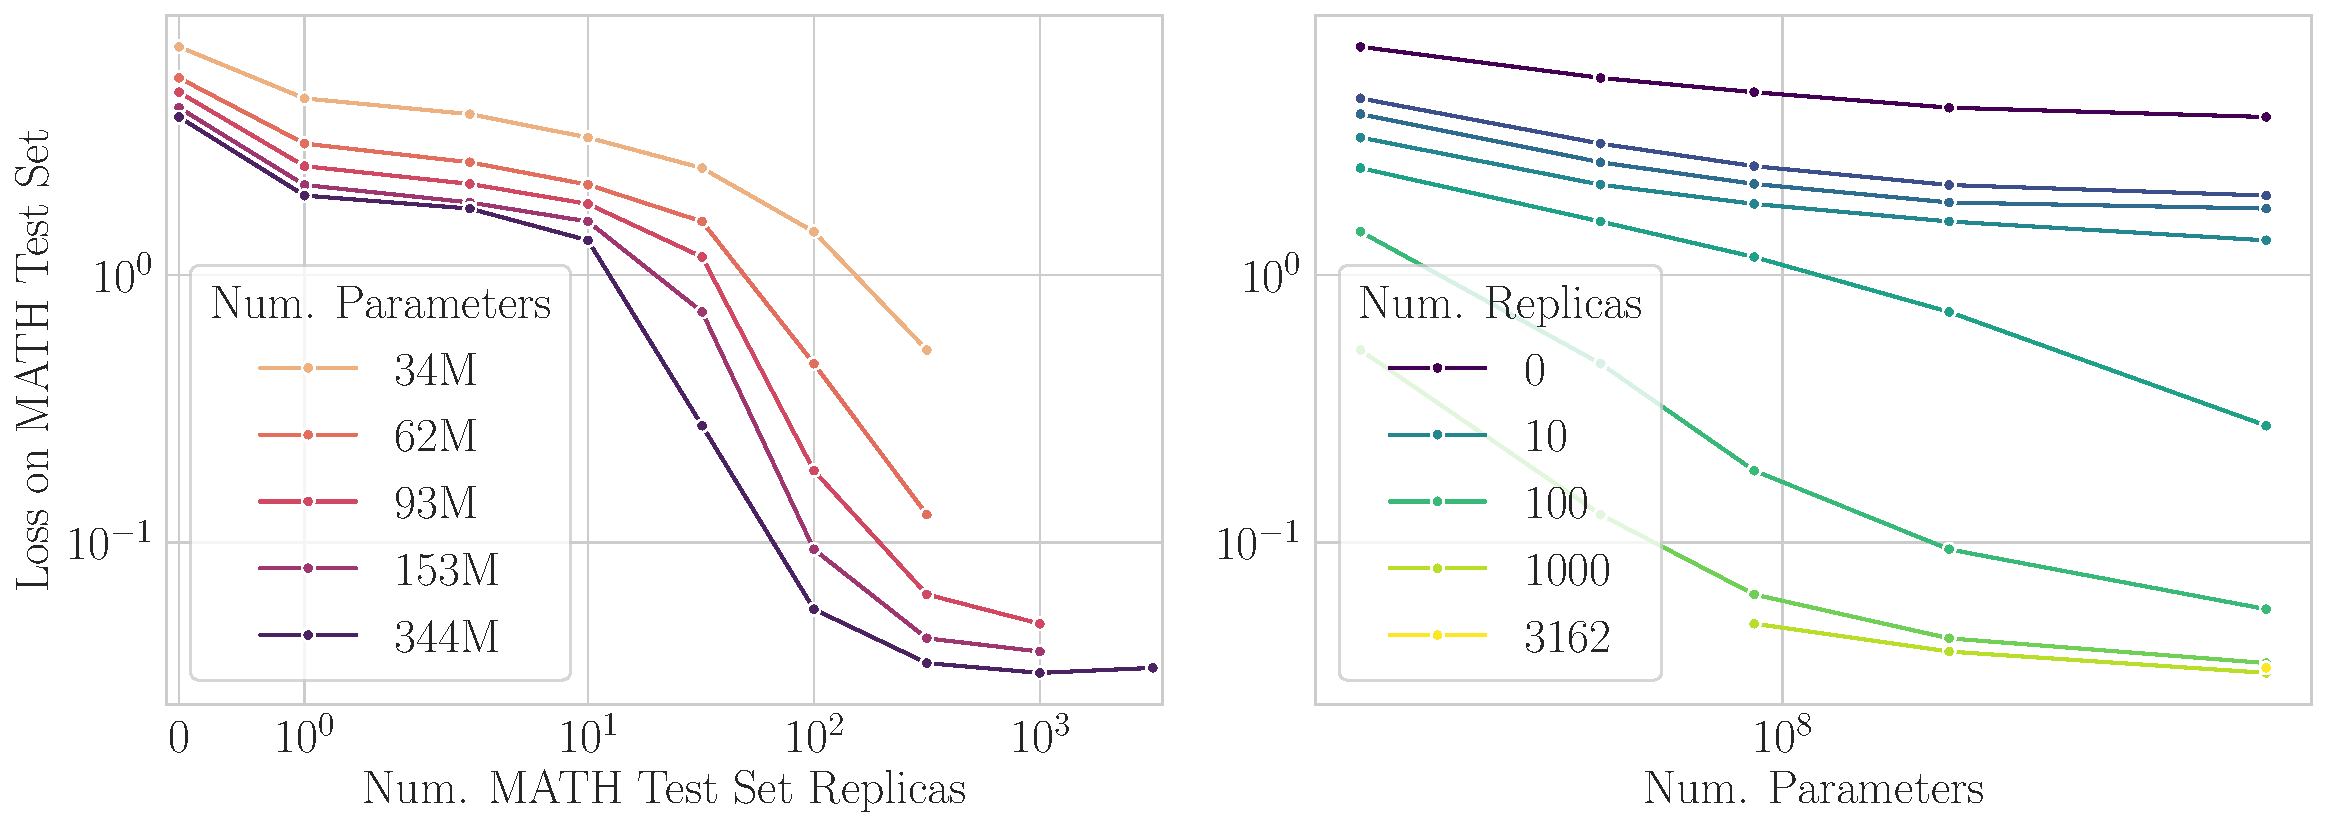
\includegraphics[width=\linewidth]{figures/10_math_qwen3_pt_cross_entropy/y=loss_by_num_parameters_by_num_replicas.pdf}
    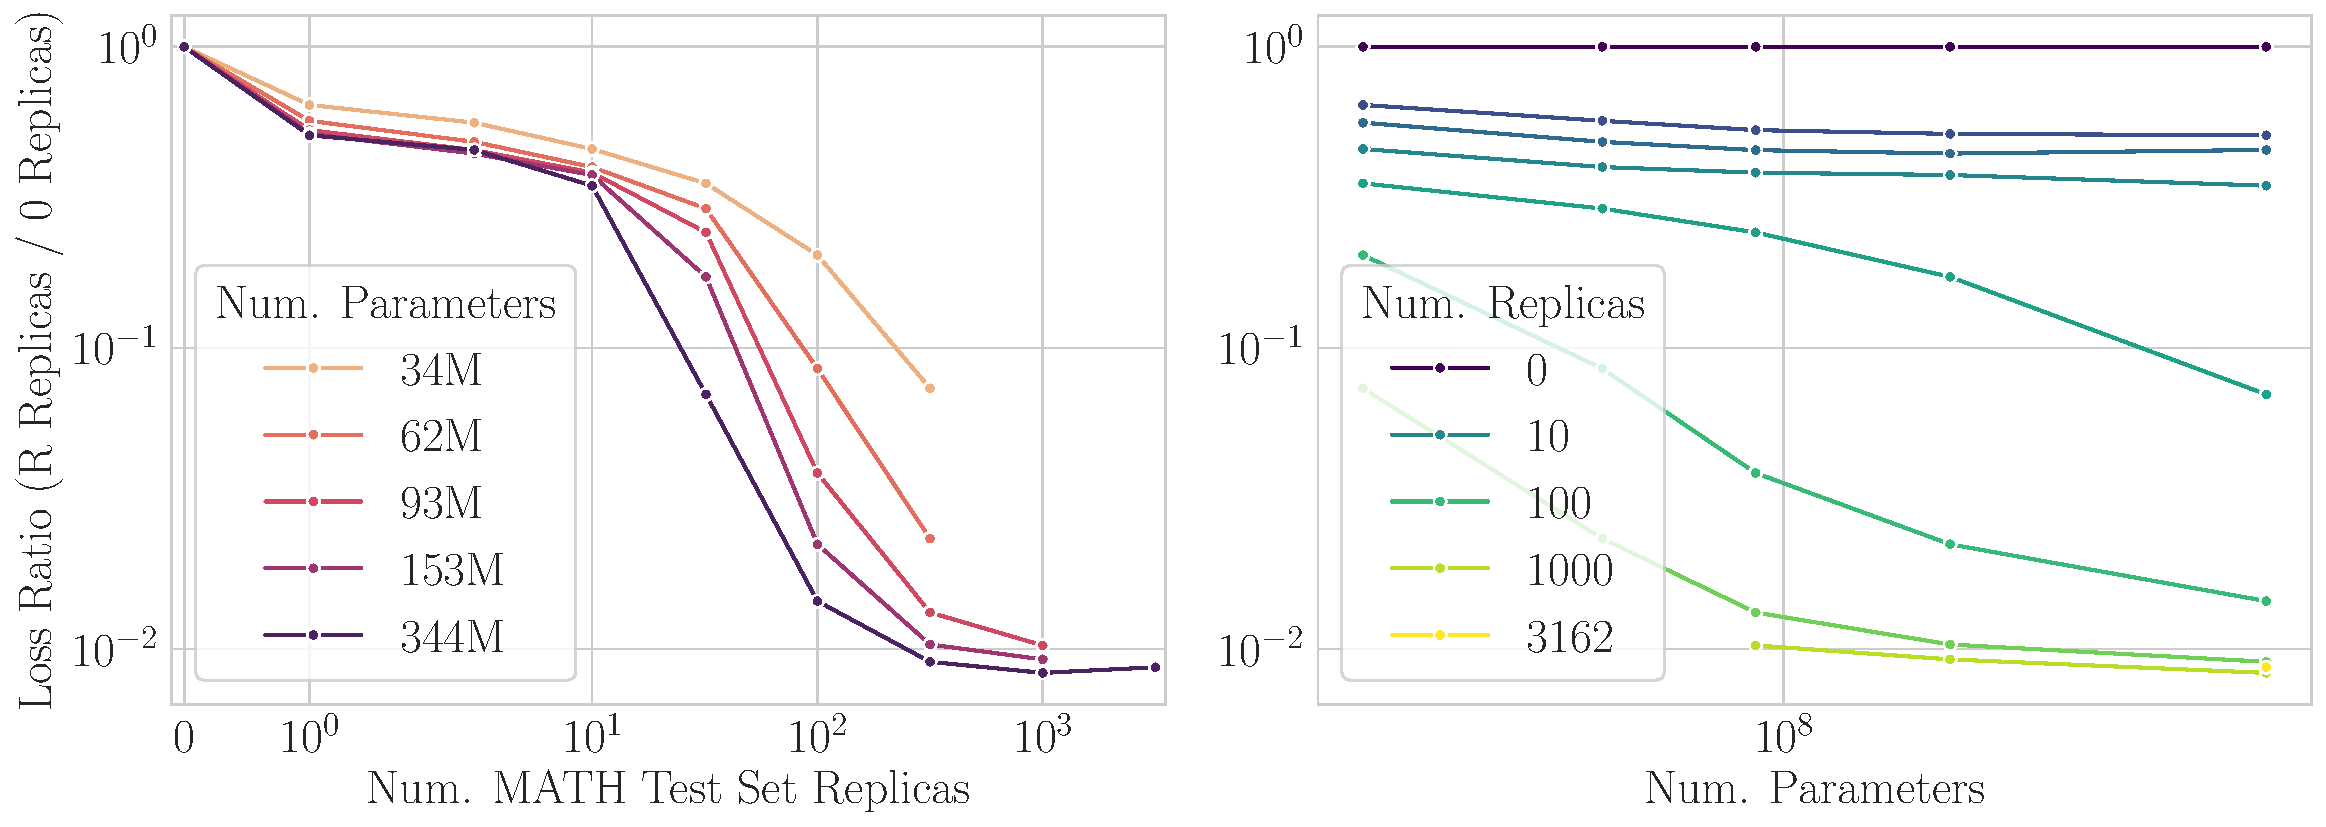
\includegraphics[width=\linewidth]{figures/10_math_qwen3_pt_cross_entropy/y=loss_ratio_by_num_parameters_by_num_replicas.pdf}
\end{minipage}
    \caption{\textbf{Performance on Generative Benchmarks Increases with Test Set Contamination and Model Size.} We pretrained compute-optimal language models ($34$M--$344$M parameters) on corpora containing $0$--$3162$ replicas of the MATH test set, then evaluated with greedy decoding. As contamination grows, Math Verify scores rise (top) and test-set cross entropies fall (bottom), with sharp improvement around $100$ replicas. The ratio of test-set loss at $R$ replicas to loss at $0$ replicas grows with model size, so larger models benefit more from contamination at any replica count.
}
    \label{fig:math_verify_ce_temp_0}
\end{figure*}

While foundational, these investigations have predominantly focused on \textit{discriminative} benchmarks like classification or multiple-choice question-answering (MCQA). For example, \citet{magar2022data} used SST-2 \citep{socher2013sst} (classification). \citet{jiang2024investigatingdatacontaminationpretraining} used SST-2 (classification), MMLU \citep{hendrycks2021measuring} (MCQA), SQuAD \citep{rajpurkar2016squad} (MCQA), and CNN/Daily Mail (fill-in-the-middle) \citep{nallapati2016abstractive}. \citet{oren2023proving} used 7 MCQA benchmarks and 1 mathematical problem solving benchmark (GSM8K) \citep{cobbe2021trainingverifierssolvemath}, and \citet{yao2024data} used 3 MCQA benchmarks while \citet{bordt2025howmuch} used 7 MCQA benchmarks.

However, with the advancement of capabilities and the advent of reasoning models \citep{openai2024openaio1card,comanici2025gemini25pushingfrontier,xu2025largereasoningmodelssurvey}, the field is shifting towards benchmarks for which the model must generate an answer rather than choose between choices.
Whether test set contamination has the same effect on \textit{generative evaluations} is unclear.
Discriminative evaluations typically require the model to place higher probability mass on the correct choice than on a few incorrect choices \citep{gao2024evalharness, schaeffer2025elusive}, and candidate choices are often only a few tokens long.
In contrast, generative evaluations require the model to produce tens-to-thousands of tokens without straying from the memorized solution, and introduce new considerations such as the sampling temperature \citep{ackley1985learning}, the sampling algorithm (e.g., top-k \citep{fan2018topk}, top-p \citep{holtzman2020topp}) and the solution length.


\begin{figure*}[t!]
    \centering
    
\includegraphics[width=0.9\linewidth]{figures/20_gen_eval_contamination_vs_compute/y=loss_x=flop_hue=num_replicas.pdf}
    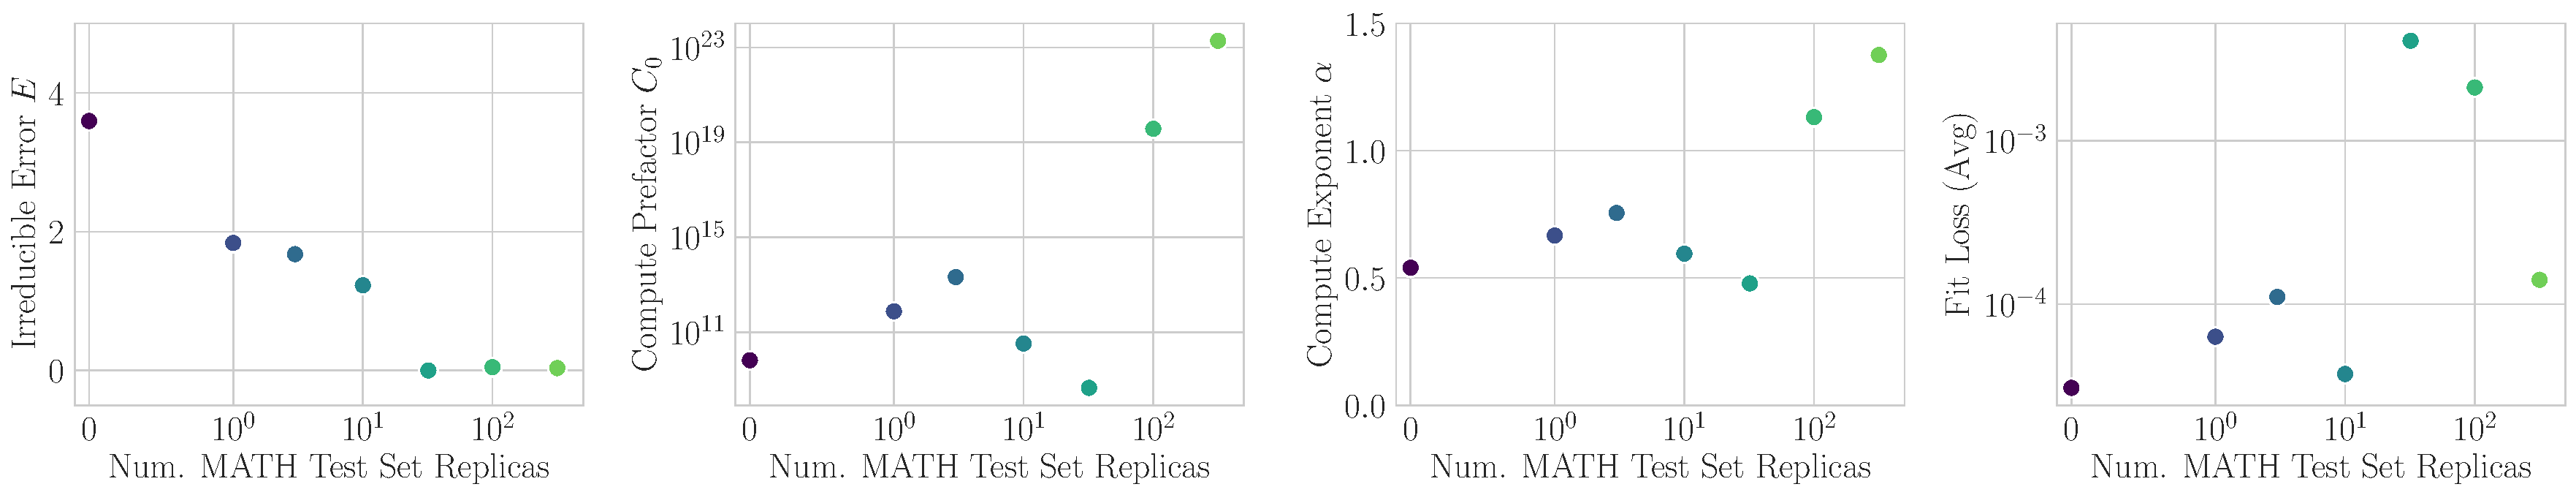
\includegraphics[width=\linewidth]{figures/20_gen_eval_contamination_vs_compute/y=fit-params_x=num-replicas_col=param_setting=full-fits.pdf}
    \caption{\textbf{Scaling Laws Suggest Including A Single Test Set Replica Achieves Lower Loss Than the Irreducible Error of the Uncontaminated Corpus.} \textbf{Top:} For each scaling series contaminated with $R$ replicas of the MATH test set, we fit scaling laws $\mathcal{L}(C, R) = E(R) + C_0(R) \cdot C^{-\alpha(R)}$, where $C \approx 6 N D$ is pretraining compute. 
    Almost all contaminated models achieve lower cross entropy on the test set than the irreducible error of training on uncontaminated data (horizontal purple line).
    \textbf{Bottom:} Increasing test set contamination reduces the irreducible error $E(R)$ from $3.594$ at $R=0$ to $0.0347$ at $R=316$. Larger values of $R$ also increase the compute prefactor and compute exponent.
    The functional form achieves average fitting error $< 10^{-2}$ for all $R$.
    }
    \label{fig:contamination_scaling_laws}
\end{figure*}

In this work, we quantitatively study the effects of test set contamination on generative evaluations, focusing on the widely used MATH benchmark \citep{hendrycks2021measuringmathematicalproblemsolving}. 
We pretrain dozens of language models on corpora contaminated with varying numbers of test set replicas, then study the effects of contamination through the language model lifecycle:

\textbf{Pretraining: Scaling \& Irreducible Error} (Sec.~\ref{sec:pretraining}). We find that performance increases with contamination and model size, similar to discriminative settings. Under standard scaling law assumptions, we discover a fundamental breach: including even a single replica of the test set enables achieving a lower loss than the irreducible error of the uncontaminated corpus.
    
\textbf{Subsequent Training: Overtraining \& Supervised Finetuning} (Sec.~\ref{sec:further_training}). We find that training beyond compute-optimal with fresh data dilutes the performance gains from contamination. We further discover that Supervised Finetuning (SFT) has opposing effects depending on pretraining contamination: it improves (worsens) performance for low (high) contamination.

\textbf{Deployment: Temperature \& Solution Length} (Sec.~\ref{sec:inference}) Sampling temperature and solution length modulate memorization, leading us to mathematically characterize three regimes: Exponentially Fast Decoherence, Brittle Memorization, and Deterministic Lock-In. We show that high-temperature sampling acts as a "truth serum," decoupling contamination gains from generalization.

As an final and general contribution, we discover and fix a critical implementation error in the EleutherAI LM Evaluation Harness \citep{gao2024evalharness} for Math Verify Scores (Appendix~\ref{app:sec:math_verify_bug}), ensuring that valid reference solutions are accurately scored as correct (raising scores of gold references from $\mathord{\sim}$70\% to 100\%), a necessary step for trustworthy reporting on mathematical benchmarks.
